\documentclass[mathserif]{beamer}

\usepackage[utf8]		{inputenc}
\usepackage[T1]			{fontenc}
\usepackage				{lmodern}
\usepackage				{amsmath}
\usepackage				{amssymb}
\usepackage				{microtype}
\usepackage             {color}
\usepackage             {mathtools}
\usepackage             {amsthm}
\usepackage             {natbib}
\usepackage             {hyphenat}
\usepackage[font=small] {caption}
\usepackage             {bbm}
\usepackage             {hyperref}
\usepackage{mathrsfs}
\usepackage				{listings}
\usepackage				{color}
\usepackage             {graphicx}

\linespread{1.3}
\beamertemplatenavigationsymbolsempty
\setbeamertemplate{footline}[frame number]

\title{FEM}
\author{Sebastian Müller, Fritz Schelten}
\date{Juni 19, 2017}


\begin{document}

\begin{frame}
\titlepage
\end{frame}

\begin{frame}
\frametitle{Überblick}
\tableofcontents
\end{frame}

\section{Ansatz function space}

\begin{frame}
	\frametitle{Basisfunctions, Shapefunctions}
	\framesubtitle{Triangle elements}
	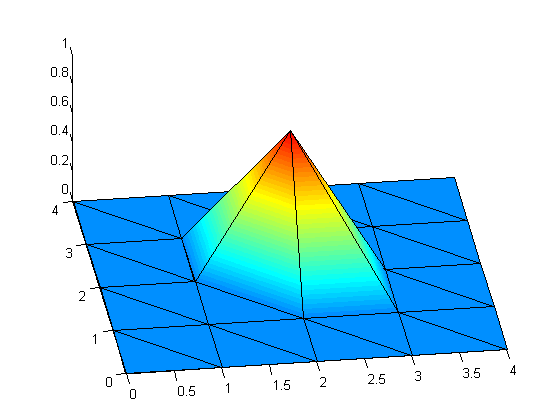
\includegraphics[height=4cm]{triangleplot.png}
	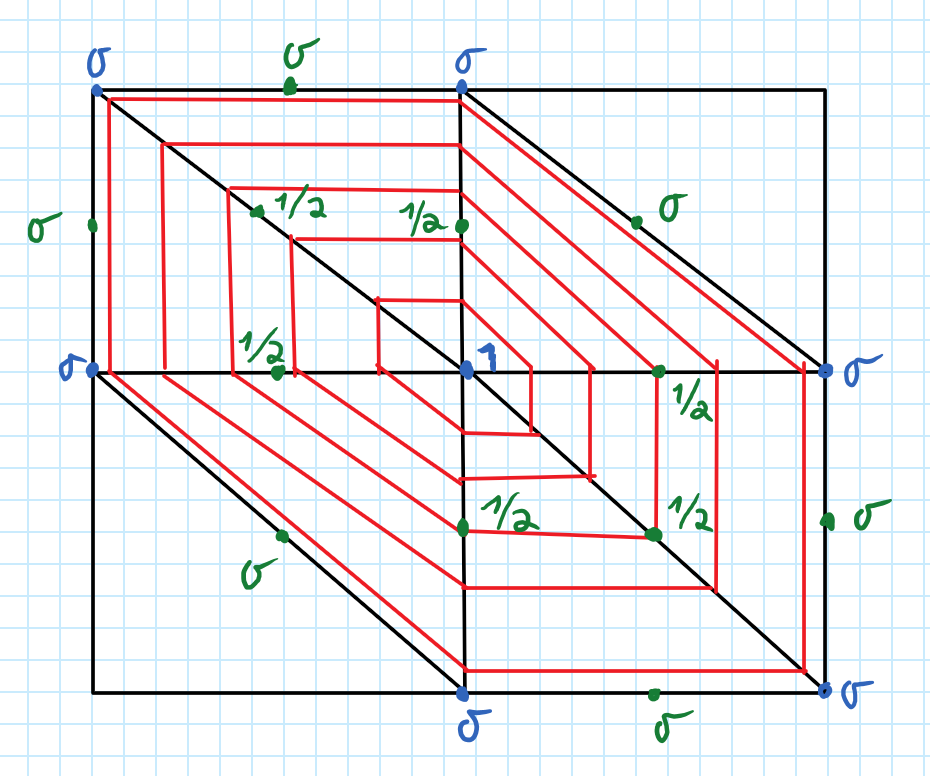
\includegraphics[height=4cm]{triangles.PNG}
\end{frame}

\begin{frame}
	\frametitle{Basisfunctions, Shapefunctions}
	\framesubtitle{Square elements}
	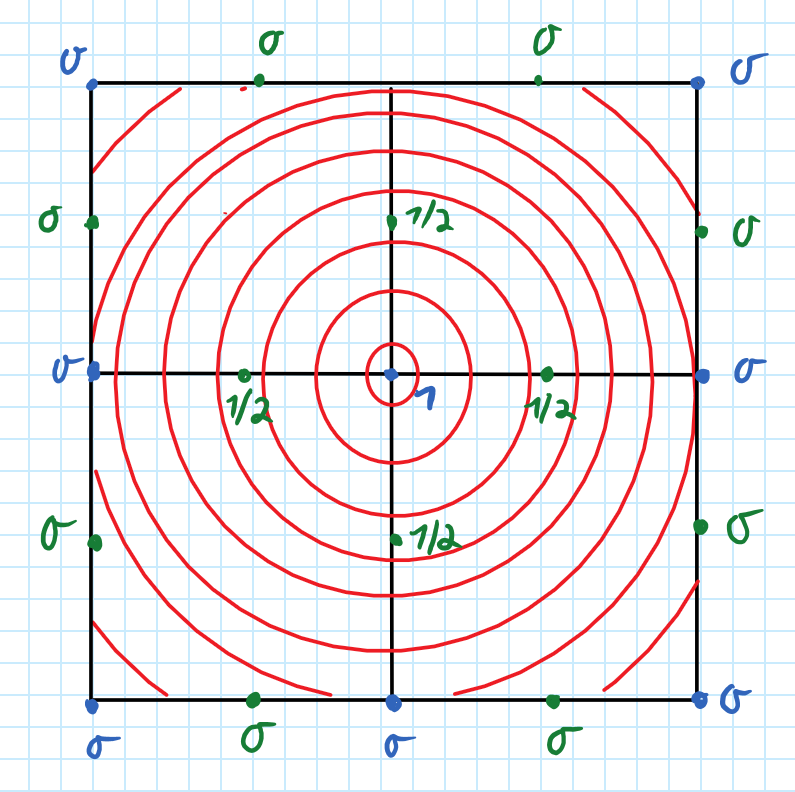
\includegraphics[height=4cm]{squares.PNG}
\end{frame}

\section{Stiffness Matrix}

\begin{frame}[fragile]
\frametitle{Stiffness matrix}
\framesubtitle{Calculation for rect. triangles and squares}
\begin{lstlisting}[basicstyle=\tiny, mathescape]
for all $\nabla \varphi_i$
  for all $\nabla \varphi_j = \nabla \varphi_1, \ldots, \nabla \varphi_i$
    $a_{ij}$ = 0
    if basis nodes of $\varphi_i$, $\varphi_j$ are neighbours
		for all shape functions $s_i$ of $\nabla \varphi_i$
		  for all shape functions $s_j$ of $\nabla \varphi_j$
		  if (domain($s_i$) == domain($s_j$))
		    $a_{ij}$ = $a_{ij}$ + $\int_{d(s_i)} \nabla \varphi_i \cdot \nabla \varphi_j (+ \varphi_i \cdot \varphi_j)dx$;
		  end
		end
	end
    A(i,j)=A(j,i)=$a_{ij}$;
  end
end
\end{lstlisting}
all gradients of basis functions are calculated before
\end{frame}

\begin{frame}[fragile]
	\frametitle{Stiffness matrix}
	\framesubtitle{Calculation for arb. triangles}
	\begin{lstlisting}[basicstyle=\tiny, mathescape]
for all $\nabla \varphi_i$
  for all $\nabla \varphi_j$
    $a_{ij}$ = 0
	for all shape functions $s_i$ of $\nabla \varphi_i$
	  for all shape functions $s_j$ of $\nabla \varphi_j$
	    if (domain($s_i$) == domain($s_j$))
	      $a_{ij}$ = $a_{ij}$ + $\int_{d(s_i)} \nabla \varphi_i \cdot \nabla \varphi_j (+ \varphi_i \cdot \varphi_j)dx$;
	    end
	  end
	A(i,j)=$a_{ij}$;
  end
end
\end{lstlisting}
all gradients of basis functions are calculated before
\end{frame}

\section{Solution}

\begin{frame}[fragile]
	\frametitle{Evaluation of solution}
	\framesubtitle{for rectangular triangles}
	Class solution assembles a shape function for each domain by summing up weighted corresponding shape functions of all basis functions.\\
	Evaluation is done by detecting the domain related to $(x,y)$
\begin{lstlisting}[basicstyle=\tiny, mathescape]
interval = ceil($x/nodeDistance_x; y/nodeDistance_y$)
domainIndex = $2 \cdot [((interval_y-1) \cdot meshIntervals_y) + interval_x]$
u = solution.shapeScalarFunctions(domainIndex).evaluate(x,y);
if (u == 0) then u = solution.shapeScalerFunctions(domainIndex-1).evaluate(x,y);
\end{lstlisting}
\end{frame}

\begin{frame}[fragile]
	\frametitle{Evaluation of solution}
	\framesubtitle{for squares}
	Class solution assembles a shape function for each domain by summing up weighted corresponding shape functions of all basis functions.\\
	Evaluation is done by detecting the domain related to $(x,y)$
	\begin{lstlisting}[basicstyle=\tiny, mathescape]
	interval = ceil($x/nodeDistance_x; y/nodeDistance_y$)
	domainIndex = $((interval_y-1) \cdot meshIntervals_y) + interval_x$
	u = solution.shapeScalarFunctions(domainIndex).evaluate(x,y);
	\end{lstlisting}
\end{frame}

\section{Errors and error estimators}

\begin{frame}
	\frametitle{A posteriori estimator}
	\framesubtitle{Calculation}
	
$r_K(u_h) := (f+ \nabla u_h)\vert_K$ and $r_E(u_h) := \left[\eta_E \cdot \nabla u_h \right]_E$
	
$\eta := \left[\sum_K \eta_K^2 \right]^{1/2}$, where $\eta_K^2 := h_K^2 \Vert r_K^2 \Vert_{0,K}^2 + \frac{1}{2} \sum_{E \subset K} h_E \Vert r_E \Vert^2_{0,E}$

where $K$ are domains and $E$ are edges.\\
This uses the shape scalar function array of the solution.	
	
\end{frame}



\end{document}
